% Template for ICASSP-2010 paper; to be used with:
%          mlspconf.sty  - ICASSP/ICIP LaTeX style file adapted for MLSP, and
%          IEEEbib.bst - IEEE bibliography style file.
% --------------------------------------------------------------------------
\documentclass{article}
\usepackage{amsmath,graphicx,02471}

%%%%%%%%%%%%%%%%%%%%%%%%%%%%%%%%%%%%%%%%%%%%%%%%%%%%%%%%%%%%%%%%%%%%%%%%%%%%%%%%
% Zach Added packages
\usepackage{acronym}
\newacro{MIDI}{musical instrument digital interface}
\newacro{NMF}{non-negative matrix factorization}
\newacro{KSVD}{k-singular value decomposition}
\newacro{NKSVD}{non-negative k-singular value decomposition}
\newacro{MAP}{maximum a-priori}
\newacro{STFT}{short time Fourier transform}
\newacro{OMP}{orthogonal matching pursuit}
\newacro{FFT}{fast Fourier transform}
\newacro{LS}{least squares}

\usepackage{todonotes}
\usepackage{minted}
\usemintedstyle{solarizedlight}
\usepackage{algorithm}
\usepackage{siunitx}
\usepackage{hyperref}
\hypersetup{
	colorlinks=true,
	urlcolor=blue
}
%%%%%%%%%%%%%%%%%%%%%%%%%%%%%%%%%%%%%%%%%%%%%%%%%%%%%%%%%%%%%%%%%%%%%%%%%%%%%%%%



\toappear{02471 Machine Learning for Signal Processing}


% Example definitions.
% --------------------
\def\x{{\mathbf x}}
\def\L{{\cal L}}

% Title.
% ------
\title{Towards Time-domain Piano Music Transcription using K-SVD}
%
% Single address.
% ---------------
\name{Zachary Neveu}
\address{Technical University of Denmark}

\begin{document}
%\ninept
%

\maketitle
%
\begin{abstract}
This work presents a method for transcribing piano music in the time domain using \ac{KSVD} given existing note onsets. The method presented allows for learning from small datasets and offers the potential to generalize to instruments with widely varying spectral characteristics and non-western musical scales.

\end{abstract}
%
\begin{keywords}
K-SVD, Factor Models, Music
\end{keywords}

code at: \href{https://github.com/zacharyneveu/MLSP\_Project}{https://github.com/zacharyneveu/MLSP\_Project}
%
\section{Introduction}
\label{sec:intro}
Music, in general, has a well defined structure that can be represented in simple forms such as sheet music or \ac{MIDI} scores. In these compressed forms, the salient features of music (note pitches, velocities, and timing) are stored directly, and can be searched and manipulated easily. Musical performance often deviates in interesting ways from written music, however live performances are most often recorded in audio form and require significant human effort to analyze or manipulate. Transforming music from a high-dimensional audio signal into a sparse symbolic form can be performed algorithmically which can save time and effort.


\section{Background}%
\label{sec:background}
Traditional signal processing approaches can perform transcription for certain musical instruments and styles with a moderate level of success \cite{klapuri_signal_2004} . These approaches generally utilize the fact that a musical note is written as the lowest frequency ($F_0$) that occurs when this note is played. In the subtask of melody transcription, it is known that only one note can occur simultaneously, so simply finding the lowest prominent frequency in the time-frequency domain can often be adequate to transcribe a sample. In polyphonic transcription, however, multiple notes can be played at once. This problem can be approached well in a statistical context using \ac{MAP} estimation to determine the most likely combination of notes occurring given a set of frequencies \cite{emiya_multipitch_2010}. Another approach to polyphonic transcription is to factor the magnitude spectrogram of the signal. Because of the nature of the \ac{STFT}, the magnitude of each time-frequency bin must be non-negative, so non-negative matrix factorization has been applied by \cite{smaragdis_non-negative_2003}. For piano music, another known constraint is that representations are sparse in the frequency domain. To utilize this, \cite{bertin_blind_2007} used \ac{NKSVD} in the spectrogram domain to constrain the sparsity of solutions along with the positivity constraint. More recently, neural networks have been applied to the polyphonic transcription task, most notably in \cite{hawthorne_onsets_2018}. Neural network approaches are able to benefit from learning musical structure, grasping the nonlinear relationships between notes over time, making them the most performant approach for polyphonic transcription. Neural architectures suffer from the lack of large-scale labeled data in this area, however, so highly general networks for multiple instruments and styles do not exist.


\section{Problem Formulation}%
\label{sec:problem_formulation}
For the purposes of this paper, it is assumed that a method for onset detection such as the one presented in \cite{bock_evaluating_nodate} is available and performs well.  The input for the problem is then time-domain frames of music each of which contains one or more onsets located exclusively at the beginning. The goal is to factor a set of frames, $X$, into an approximate linear combination, $Z$, of a dictionary of notes, $\mathbf{D}$, as expressed in equation \eqref{eq:factor}. The dimensionality of the variables are $X \in R^{n\times N}$, $D\in R^{n\times K}$, and $Z \in R^{K \times N}$ where $N$ is the number of audio frames, $n$ is the length of a frame, and $K$ is the number of atoms in the dictionary. The constraint is imposed that the number of non-zero elements in $Z \le k$ where $k \ll K$. For our specific purposes $K$ was chosen to be $88$ because a piano has $88$ possible notes, and $k$ was chosen to be $10$ as the average pianist has $10$ fingers. Solving for $\mathbf{D}$ and $Z$ exactly is an NP-hard problem, so for practical purposes results must be estimated.

\begin{equation}
\begin{tabular}{cr}
	$X \approx \mathbf{D}Z$ & $s.t.\ \|Z\|_0 \le k$
\end{tabular}
\label{eq:factor}
\end{equation}


\section{Data}%
\label{sec:data}
A subset of the MAESTRO dataset is used to fit the dictionary \cite{hawthorne_enabling_2019}. This data consists of audio files of piano music alongside \ac{MIDI} files which contain the times, frequencies, and amplitudes of each note played. These audio files are oversampled to $44,100\,Hz$  to cover the full range of human hearing, however this is  generally unnecessary for music transcription (the highest piano note has an $F_0$ of $4186\,Hz$), so the audio files were downsampled by a factor of $4$ to $11,025\,Hz$. Using the \ac{MIDI} annotations, audio files were then split at note onsets. Each frame was then zero-padded or cropped so that the length of all frames was identical and of a tractable size of $512$ samples. These frames were then concatenated into a $N\times 512$ matrix suitable for training the dictionary.



\section{Algorithm}%
\label{sec:algorithm}
The \ac{KSVD} algorithm was originally introduced in \cite{aharon_k-svd_2005} and provides a way to learn an over complete dictionary with which to represent signals with a given sparsity. Listing 1 shows an overview of the \ac{KSVD} algorithm for signal X, dictionary D and a given maximum number of iterations. Essentially, the algorithm is an iterative process with two parts. First a sparse combination of dictionary atoms is found that best fit the signal using the \ac{OMP} algorithm seen in Listing 1 \cite{tropp_greed_2004}. Next, the dictionary D is updated one atom at a time so that the selected atom contributes as possible to the sparse representations of all data points which use it. These two steps are repeated either convergence or until a specified maximum number of iterations. \begin{listing}[h]
\begin{minted}[tabsize=3,escapeinside=||]{Julia}
function KSVD(X,D,max_iter)
	# Initialization
	D = random(n,K)
	for j=1:max_iter
		# Sparse Coding
		Z = OMP(X, D, k)
		# Dictionary Update
		for k=1:K
			# create error matrix
			|$E_k$| = X-(DZ-D[k]Z[k])
			|$w_k$| = ones(N, 1)
			|$w_k$|[k] = 0
			|$E_k$| = |$E_k$|[wk,:]
			D[k], Z[k] = SVD(|$E_k$|)
		end
	end
	return D, Z
end
\end{minted}
\label{lst:ksvd}
\caption{K-SVD Algorithm \cite{aharon_k-svd_2005}}
\end{listing}

\begin{listing}[h]
\begin{minted}[tabsize=3,escapeinside=||,mathescape=true]{Julia}
function OMP(X, D, max_nonzeros)
	residual = X
	active_atoms = []
	for i=1:max_nonzeros
		atom_corrs = D'*residual
		atom_idx = argmax(abs.(atom_corrs))
		push(active_atoms, atom_idx)
		selected_atoms = D[:,active_atoms]
		z = least_squares(selected_atoms, X)
		residual = residual-selected_atoms*z
	end
	return_val = zeros(n_atoms)
	return_val[active_atoms] = z;
	return return_val
end
\end{minted}
\label{lst:omp}
\caption{Orthogonal Matching Pursuit Algorithm \cite{tropp_greed_2004}}
\end{listing}

\noindent
In order to reconstruct frames after $D$ is trained, \ac{OMP} can be used without performing \ac{KSVD} after. The task of fitting $Z$ given $X$ and $D$ is NP-Hard. \ac{OMP} is an iterative greedy algorithm that gives very good approximate results. The premise behind \ac{OMP} is to select atoms that are most correlated to the parts of the input signal not yet represented by chosen atoms. First, the most correlated atom is chosen, and its weight is fit using \ac{LS}. The weighted atom is then subtracted from the residual and the process is repeated. The benefit to using this approach over the original approach to matching pursuit introduced by \cite{mallat_matching_1993-2} is that using  \ac{OMP}, the atoms are chosen to be orthogonal. This means that instead of choosing two atoms and two weights to represent an aspect of the signal, \ac{OMP} will instead choose a larger weight, freeing up an atom to be used for another purpose.




\section{Results}%
\label{sec:results}
To evaluate the results of KSVD, the learned dictionary atoms, as well as example signal reconstructions are examined. For the specific task at hand, it is known that piano music is sparse in the frequency domain, so the dictionary atoms should have learned meaningful frequency-domain content. To evaluate this, the \ac{FFT} of each atom was calculated. Figure \ref{fig:figs-atoms-png} shows the magnitudes of the \ac{FFT} for each atom sorted by the frequency of maximum component. From figure \ref{fig:figs-atoms-png}, it is clear that \ac{KSVD} has learned the primary frequencies of a variety of notes. It is important to note that the training data does not necessarily include every note on a piano, and this may be the reason that certain notes have multiple atoms while others do not have an atom. To evaluate the reconstructed data, several audio frames not seen in the training dataset are reconstructed using the learned dictionary and the \ac{OMP} algorithm. Figure \ref{fig:figs-reconstructed-png} shows a subset of one of these frames, approximated using 10 atoms, as well as all atoms from the dictionary.

\begin{figure}[h]
	\centering
	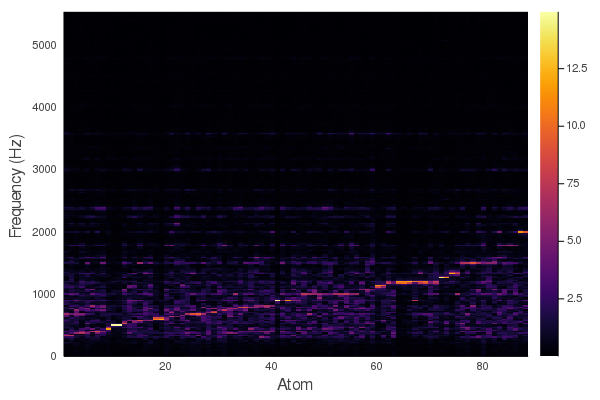
\includegraphics[width=0.5\textwidth]{figs/atoms.png}
	\caption{Learned Frequencies of Dictionary Atoms}
	\label{fig:figs-atoms-png}
\end{figure}

\begin{figure}[h]
	\centering
	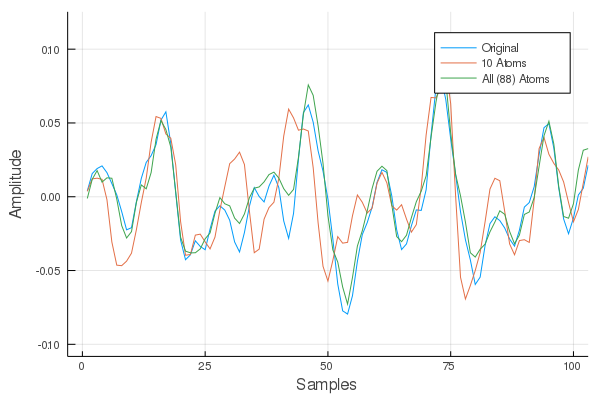
\includegraphics[width=0.45\textwidth]{figs/reconstructed.png}
	\caption{Example of Reconstructed Signal with 10 and 88 Atoms}
	\label{fig:figs-reconstructed-png}
\end{figure}


\section{Conclusions}%
\label{sec:conclusions}
The conclusions of this work are that \ac{KSVD} is capable of extracting notes from piano music in the time domain. This learning method can include a parameter specifying the maximum number of non-zero notes per frame, as well as the maximum number of possible notes to learn. These features make the technique generalizable to a large variety of instruments. One continuation of this work that could further improve performance would be to learn a complex, rather than real, vector $Z$. In the current scheme with a real value of $Z_i$, atom $D_i$ contributes best only when it has a phase of either \ang{0} or \ang{180}. Making $Z_i$ complex would allow $D_i$ to contribute more when $X$ is out of phase from the other training data. Another continuation of this work would be to pair the current algorithm with a note onset detection algorithm and measure the performance transcribing when there are some errors in the frame boundaries. Under these conditions, it would be possible to determine the extent to which this algorithm is feasible for real-world tasks.



% References should be produced using the bibtex program from suitable
% BiBTeX files (here: strings, refs, manuals). The IEEEbib.bst bibliography
% style file from IEEE produces unsorted bibliography list.
% -------------------------------------------------------------------------
\bibliographystyle{IEEEbib}
\bibliography{refs}

\end{document}
